\documentclass{article}
\usepackage[utf8]{inputenc}
\usepackage{graphicx}
\usepackage{tikz}
\usetikzlibrary{automata, positioning, arrows}
\title{Ros Software Architecture}
\author{}
\date{}
\begin{document}
\maketitle
\tikzset{
         ->,  % makes the edges directed
         >=stealth, % makes the arrow heads bold
         node distance=3cm, % specifies the minimum distance between two nodes. Change if necessary.
         every state/.style={thick, fill=gray!10}, % sets the properties for each ’state’ node
         initial text=$ $, % sets the text that appears on the start arrow
         }
\section{Intro}
Ros is an open-source robotics middleware suite. Although ROS is not an operating system (OS) but a set of software frameworks for robot software development, it provides services designed for a heterogeneous computer cluster such as hardware abstraction, low-level device control, implementation of commonly used functionality, message-passing between processes, and package management. (stole definition from Wikipedia)

\section{Publisher Subscriber Architecture Model}
\begin{figure}[htp]
    \centering
    \includegraphics[width=12cm]{pubsub.png}
    \caption{}
    \label{fig:pubsub}
\end{figure}\\\\
\textbf{Nodes:} Are usually associated with a python script or c++ object. Nodes can do two main things - publish and subscribe. A node can be both a publisher and a subscriber.\\\\
\textbf{Publisher node: } Publish(send) data to a topic(Represented by outing edges in figure above). \\\\
\textbf{Subscriber node: } Subscribes(listens) to data from a topic(Represented by incoming edges in figure above), then uses a callback function to create desired output from topic data. \\\\
\textbf{Topics: } Are the name handlers for where nodes will publish and subscribe to data.\\\\
\textbf{Ros messages: } Are objects predefined in ros or defined by the programmer that can be transmitted over topics. 
\section{System Design}
Ros programming is often done using a top to bottom approach. The engineer must design the system architecture(as shown above), then develop(code) the individual nodes of the system.\\\\
\textbf{Advantages:} \\
1. Simplifies documentation and readability of the system.\\
2. Stores code in modular nodes that can be easily added and removed to any system(increases code re-usability).\\
3. Increased programming efficiency since nodes can be written in different languages and are allowed to communicate within a ros environment.\\
4. Ros nodes communicate using asynchronous message passing, which improves performance by simplifying parallelism and making it more accessible to developers.

\section{Whats a callback function?}
Publisher nodes send data to topics, and subscriber nodes collect data from topics. Each time a subscriber node receives data from a topic, the subscriber node will run a callback function. A callback function is a function, that receives data(input) from a topic asynchronously, and computes the output in separate thread. Each time data is received from a topic a new thread opens and runs the callback function. 

\section{Whats a point cloud?}
A point cloud is a set of 3d points within some frame. Example of devices that gather point cloud data are kinect(xbox), lidar(similar to radar), and stereo camera(uses two rgb cameras to triangulate 3d points). 
\section{Example of architecture}
Design a system  architecture using the publisher-subscriber model that from 2D object inferences, the robot moves it head in 
the direction of individual people. If there is more than one person, the robot creates a list of 
centroids(representing the people) and iterates through this list by pointing its head at each person for three seconds. 
The robot has two measuring devices, a camera which outputs rgb images of what the robot is looking at, 
and a kinect device that outputs a point-cloud of 3D points measured in the same frame as the camera.\\\\\\
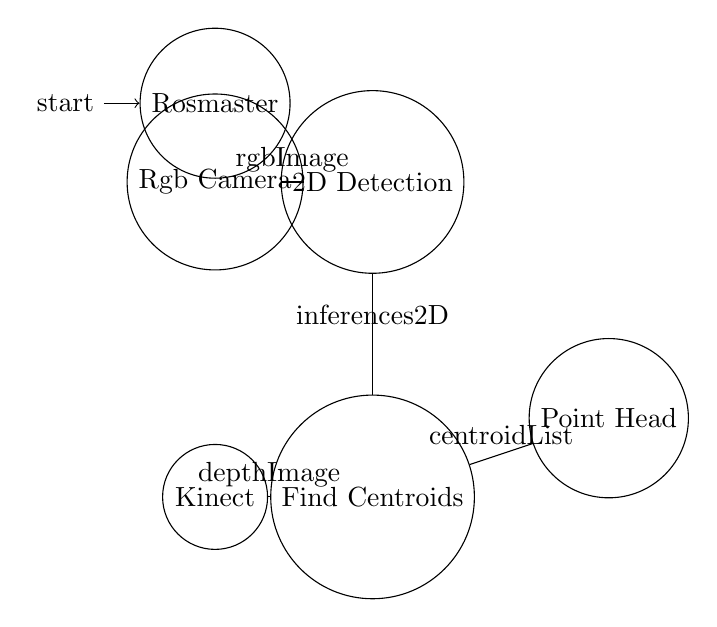
\begin{tikzpicture}
    % tikz code goes here
    \node[state, initial] (1) {Rosmaster};
    \node[state, below of=1] (2) {Rgb Camera};
    \node[state, below of=2] at (0, -4) (3) {Kinect};
    \node[state, below of=1, right of=2] at (1,0) (4) {2D Detection};
    \node[state, below of=2, right of=3] at (1,-4) (5) {Find Centroids};
    \node[state, right of=5] at (4,-4) (6) {Point Head};

    \draw   (2) edge[above] node{rgbImage} (4)
            (3) edge[above] node{depthImage} (5)
            (4) edge[above] node{inferences2D} (5)
            (5) edge[above] node{centroidList} (6);
\end{tikzpicture}
\label{fig:my_label}
\end{document}
